\documentclass{article}

\usepackage{graphicx}
\usepackage{tikz}
\usetikzlibrary{arrows}
\usetikzlibrary{quantikz}

\usepackage{physics}
\usepackage{amsthm}

\title{2QANIM: 2QAN Compiler Improved}
\author{S. S. Kahani}

\newtheorem{defn}{Definition}
\newtheorem{prob}{Problem}
\def\F{\mathcal{F}}

\begin{document}
  \maketitle
  \begin{abstract}
    { \color{blue} TODO }
  \end{abstract}

  \section{Introduction}
  
  While we are far from a general-purpose quantum computer 
  \cite{?} % maybe that 2019 paper or BCG/McKenzie?
  that speeds up solving a vast range of problems, early real-world application could still be happening anytime soon by focusing on specific problems.
  %TODO any reference?
  Therefore, the importance of specific-purpose compilation is undeniable.
  
  Moreover, it is guessed that the early applications of quantum computers will include but not be limited to discrete optimizations and physical simulations.
  \cite{?} % 2019 paper
  This means that studying the compilation of k-local Hamiltonians is a meaningful choice as they play a significant role in the optimizations (like in QAOA \cite{?} and VQE \cite{?}) and undoubtedly in the physical simulations as well. 
  \cite{?} % TODO cite some review paper

  % TODO related work
  { \color{blue} TODO related work }
  
  This work is based on the 2QAN compiler \cite{?} which is a hardware-aware compiler for 2-local Hamiltonians. The main contribution of this work is to improve the compilation of 2QAN by taking errors into account and introducing a new compilation algorithm. 

  % TODO classical compilation
  { \color{blue} TODO classical compilers }

  Here we introduce a hardware-aware compiler, starts from a 2-local Hamiltonian, defined in Definition \ref{defn:2-local-hamiltonian}, allocates qubits and generates intermediate gates that are studied in Section \ref{sec:two-qubit-gates} and finally transpile them to a lower-level gate-set. This compiler aims to reduce error in a reasonable compile-time, Therefore a detailed description of the assumed error model is given in Section \ref{sec:error-model}.

  \begin{figure}[h]
    \centering
  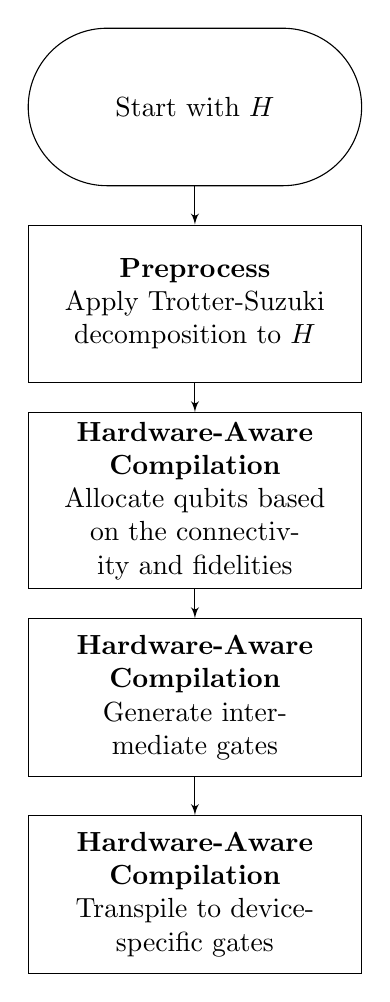
\begin{tikzpicture}[auto, node distance= 2.5cm,>=latex']
    \tikzstyle{block} = [draw, rectangle, text width=4cm, align=center, minimum height=2cm];
    \tikzstyle{rblock}=[block, rounded corners=1cm];
    \node [rblock] (a) {Start with $H$};
    \node [block, below of=a] (b) {\textbf{Preprocess} \\ Apply Trotter-Suzuki decomposition to $H$};
    \node [block, below of=b] (c) {\textbf{Hardware-Aware Compilation} \\
    Allocate qubits based on the connectivity and fidelities};
    \node [block, below of=c] (d) {\textbf{Hardware-Aware Compilation} \\
    Generate intermediate gates};
    \node [block, below of=d] (e) {\textbf{Hardware-Aware Compilation} \\
    Transpile to device-specific gates};
    \draw [->] (a) -- (b);
    \draw [->] (b) -- (c);
    \draw [->] (c) -- (d);
    \draw [->] (d) -- (e);
  \end{tikzpicture}
  \caption{The overview of the compilation process in 2QANIM}
\end{figure}

  \section{Basic Concepts}

  Because of the exponential growth of the number of gates in the compilation of a k-local term \cite{?}, setting $k=2$ is a reasonable choice for NISQ devices. This simplification not only helps us by reducing the number of gates, also enables us to use graph theory to define and analyze the problem, which is not easily possible for higher values of $k$.

  Here we introduce our notation for the Hamiltonian.

  \begin{defn}[2-local Hamiltonian]
    \label{defn:2-local-hamiltonian}
    Defining an $N$-qubit Hilbert space
    $\mathcal{H} := \otimes_{i=1}^{N} \mathcal{H_i}$, a 2-local Hamiltonian $H$ acting on it will be like
    \begin{equation}
      H := \sum_{i=1}^{k} h_i
    \end{equation}
    where each $h_i$ is a 2-local term, acting nontrivially on two specific qubits.
  \end{defn}
  \begin{defn}[Graph representation of a Hamiltonian]
    We will define the graph $G_H(V_H, E_H)$ to represent the Hamiltonian $H$, in a way that for each term $h_i$ in $H$, we have an edge $e_i$ between the two qubits it acts on.
  \end{defn}

  The very first step toward the compilation of a 2-local Hamiltonian is to apply the first-order Trotter-Suzuki decomposition \cite{?} to it. This decomposition is a way to approximate the time evolution of a Hamiltonian by a sequence of gates. 
  % TODO error of trotter

  \begin{defn}[Trotter-Suzuki decomposition]
    The first order Trotter-Suzuki decomposition, decomposes a Hamiltonian $H$, into a set of two-qubit gates $g_i$s which associated with an edge like $e_i$.
    \begin{equation}
      \text{Target Gates} := \{ (g_i, e_i) \}
    \end{equation}
  \end{defn}

  The key feature of this decomposition (only the first order) is that the resulting gates can be applied in any order. This arbitrariness is not hold for a general quantum circuit and it may cause an advantage for a problem-specific compiler. % TODO bad wording
  
  % TODO what about higher order Trotter-Suzuki decomposition?
  % TODO see the new paper "Trotter Errors and the Emergence of Chaos in Quantum Simulation"

  \section{Two Qubit Gates}
  Here we mention the two-qubit gates that are used as an intermediate gates in the process of compilations.
  
  \subsection{SWAP and Bridge Gates}
  In a situation that a mapping is already applied, the main limitation is the connectivity of the device, therefore in a case that the two qubits are not directly connected, we need to employ a chain of gates, to apply the target gate on them.

  The SWAP gate is well-known, but it is not the only gate that can be used for this purpose. The bridge gates that are introduced in \cite{?} for a simple case, can be expanded and employed for this purpose. 

  The bridge gate is an equivalent expansion of a CNOT gate, applied on two qubits that are connected through a chain of qubits.
  
  The bridge gate is defined as follows:
  \def\qceq{\midstick[4,brackets=none]{=}}
  \begin{defn}{Bridge Gate}
    \begin{figure}[h]
      \centering
 \begin{quantikz}
\qw &\ctrl{3} &\qw\qceq & \qw & \qw &\ctrl{1} & \qw & \qw & \qw & \ctrl{1}&\qw&\qw\\
\qw & \qw & \qw & \qw &\ctrl{1} & \targ{} &\ctrl{1} & \qw &\ctrl{1}& \targ{} & \ctrl{1}&\qw\\
\qw & \qw & \qw &\ctrl{1} & \targ{} & \qw & \targ{} &\ctrl{1}&\targ{} & \qw & \targ{} &\qw \\
\qw & \targ{} & \qw & \targ{} & \qw & \qw & \qw & \targ{} & \qw &\qw& \qw & \qw 
 \end{quantikz}
      \caption{The bridge gate}
    \end{figure}
    \[ \text{Bridge}(i, j) := \qty( \prod^{\leftarrow}_{k = i + 2, k < j} \text{CNOT}(k - 1, k) \prod^{\leftarrow}_{k = j, k > i} \text{CNOT}(k - 1, k) )^2  \]
  \end{defn}

  As far as we know, the family of bridge gates with more than one qubit in the chain is not studied yet, and neither implemented in any quantum compiler. 
  It can be easily shown that for a simple case like the one in the figure \ref{fig:bridge-simplification} that we need to swap and return the qubits, using bridge gate can reduce both depth and number of gates. { \color{red} DOUBT } % TODO

  \begin{figure}
    a) \\
    \begin{center}
    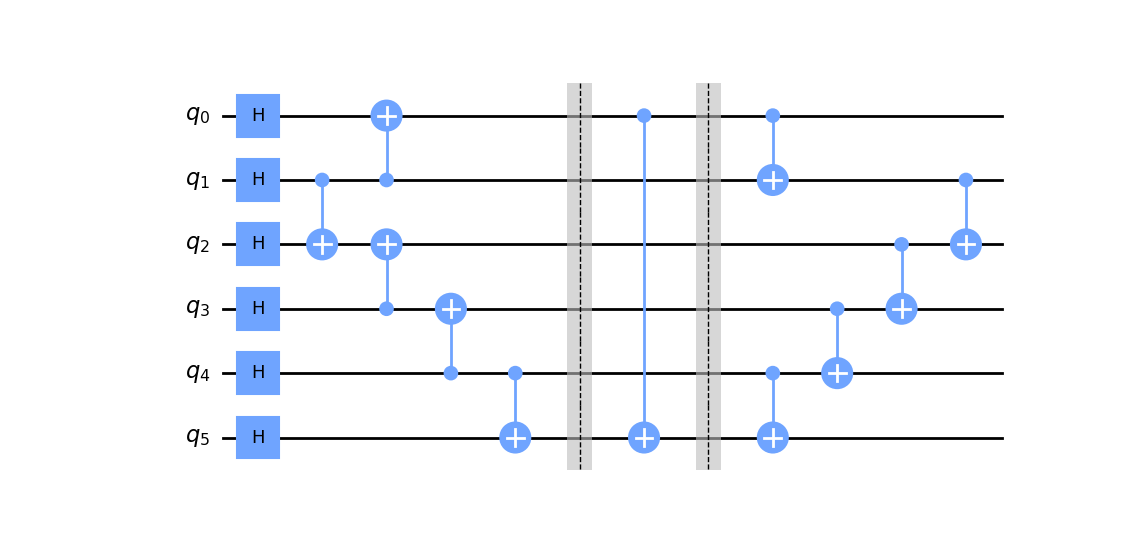
\includegraphics[width=0.9\textwidth]{../code/expm_1_bridge/out/original_circuit}
    \end{center}
    b) \\
    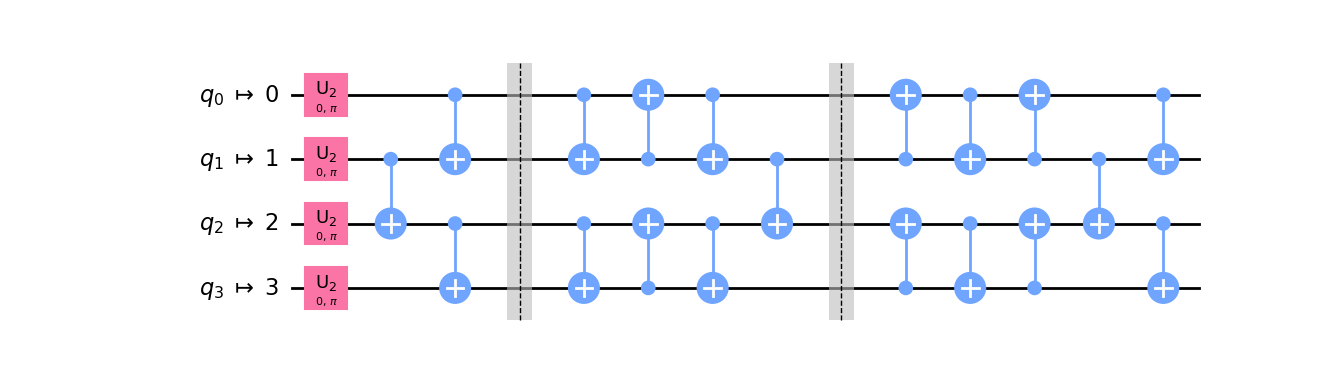
\includegraphics[width=0.9\textwidth]{../code/expm_1_bridge/out/transpiled_circuit_swap} \\
    c) \\
    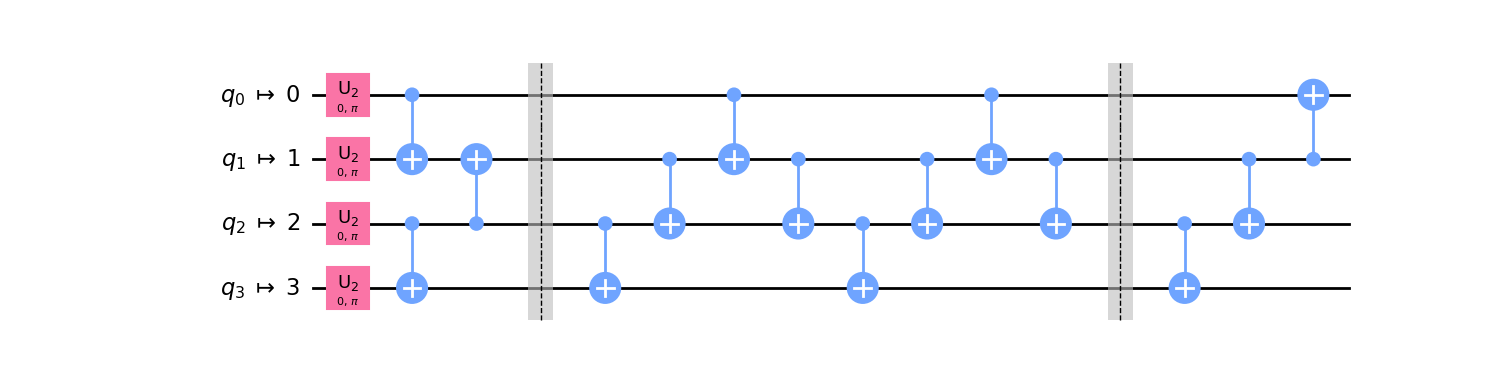
\includegraphics[width=0.9\textwidth]{../code/expm_1_bridge/out/transpiled_circuit_bridge}
    \caption{a) The original circuit, consisting of some local operations, then a far away CNOT and then some local operations. b) The circuit after transpiling using Qiskit. c) The circuit after transpiling using bridge gate as an intermediate gate.}
  \end{figure}
  \subsection{Unifying Gates}

  { \color{blue} TODO }
  We can combine two-qubit gates...

  \section{Error Model}
  \label{sec:error-model}
  Here we introduce a model to estimate errors of a circuit on a device.
  In this model, we take the average infidelity of a circuit as a measure of the error. In order to calculate the average (in)fidelity, we consider two different source of errors.

  \begin{itemize}
    \item \textbf{Decoherence}: When a qubit is left alone for some amount of time, it will decay to a random state. The average fidelity of the qubit can be written as:
    \begin{equation}
      \label{eq:decoherence}
      F_\text{decoherence}(t) = \exp(-\frac{t}{\tau_\text{decoherence}})
    \end{equation}
    \item \textbf{Gate Errors}: Any gate, specially the two-qubit gates, are not perfect. We can assign an average fidelity to each gate.
  \end{itemize}

  As for any parallel or sequential processes, the average fidelity of the circuit is the product of the average fidelity of each process, we use $-\log \F$, as a positive measure of error with additivity.

  Therefore, a device is defined as a tuple of the following:
  
  \begin{defn}[Device]
    \[ \text{Device} := (w_0 , G_d(V_d, E_d, w_\F)) \]
    where
    \[ \begin{cases}
    w_0 = \tau_\text{2-qubit gate time} / \tau_\text{decoherence}   \\ 
    w_\F(e) = -\log(\bar\F_\text{2-qubit gate on edge $e$} ) 
    \end{cases} \]
  \end{defn}
  
  \section{Problem Formulation}

  \subsection{NP-Hardness}
  Anyhow we define the problem, it is inevitable to have a subproblem like below

  \begin{prob}[Qubit Allocation]
    Given a graph that represents a Hamiltonian $G_H(V_H, E_H)$, find an allocation $\phi : V_H \to  V_d$ such the maximum number of edges in $E_H$ are mapped to $E_d$.
  \end{prob}

  We may use any other more complex criteria, such as minimizing estimated circuit error or minimizing the number of gates in the implemented circuits. But even in the simplest case, the problem is NP-hard, as the graph isomorphism problem can be reduced to it \cite{?}.

  But yet, this argument could be easily misinterepted into the fact that it is impossible to address the exact compilation algorithm in any case. It states that for an abitrary device graph, the problem is NP-hard. If we just add a simple constraint that the device graph has a bounded degree, then the problem is solvable in polynomial time. \cite{?}
  % TODO
  % TODO what about linear/lattice graph?

  \subsection{General Treatment}
  % TODO
  
  \section{Algorithms}
  \subsection{2QAN}
  \subsection{A*}
  % branching, consistency, admissibility
  \subsection{Resource Allocation}
  
\end{document}